\documentclass[paper=a4, fontsize=11pt]{scrartcl}
\usepackage{enumerate}
\usepackage{amsmath}
\usepackage{amssymb}
\usepackage{tikz}
\newcommand{\parens}[1]{ \left( #1 \right) }
\begin{document}
\noindent Willy Xiao and Kevin Eskici \\ STAT 221 \\ Oct 22, 2014
\begin{enumerate}[\text{question }1.]
  \item Show: \\
    \begin{enumerate}[(a)]
      \item \begin{align*}
        E\left[ \nabla l(\theta; y) \right] &= 0 \text{ at }\theta^* \\
        \nabla l(\theta; y) &= \frac{(y - b'(x^T\theta^*))*x}{\phi} \\
        E\left[ \frac{y_n - b'(x^T\theta^*)}{\phi} \right] &= \frac{E(Y) - b'(x^T\theta^*)}{\phi} = 0 \\
        E(Y) &= b'(x^T\theta^*)
      \end{align*}
      \item \begin{align*}
        \text{ We know that } -E\left[ \nabla \nabla l(\theta; y) \right] &= E\left[ \nabla l(\theta; y) \right]^2 \\
        \nabla \nabla l(\theta; y) &= \frac{-b''(x^T\theta^*)}{\phi} \\
        E\left[ \frac{Y - b'(\lambda)}{\phi} \right]^2 &= \frac{E(Y - E(Y))^2}{\phi^2} = \frac{Var(Y)}{\phi^2} \\
        \phi b''(\lambda_n) = \phi h'(\lambda_n) &= var(y_n|\lambda_n)
      \end{align*}
      \item \begin{align*}
        l(\theta; y) &= \frac{\lambda_ny_n - b(\lambda_n)}{\phi} + \log{y_n, \phi} \\
        \nabla l(\theta, y) &= \frac{1}{\phi}*(y_n - b'(x^T\theta))x_n \\
          &= \frac{1}{\phi}*(y_n - h(x^T\theta))x_n
      \end{align*}
      \item This is the fisher's information:
        \begin{align*}
          - \nabla \frac{1}{\phi}*(y_n - h(x^T\theta))x_n &= \nabla \frac{1}{\phi}*h(x^T\theta)x_n \\
          I(\theta) &= \frac{1}{\phi} E(h'(x^T\theta)x_nx_n^T)
        \end{align*}
      \item Because we know the fisher's information must be positive (it's a variance) and we know that $x_nx_n^T$ is positive-definite, then that means $h'(x^T\theta)$ must also be positive. If this is true then it means $h(\cdot)$ is non-decreasing.
    \end{enumerate}
  \item Experiment: \\
    \begin{enumerate}[(a)]
      \item
        \begin{align*}
          \text{ SGD: } \theta_{t+1} &= \theta_t + (1 + .02*t)^{-1}*(\Sigma^{-1}*(\vec{x_t} - \vec{ \theta_t})) \\
          \text{ ASGD: } \overline{\theta}_{t+1} &= (1 - 1/t)*\overline{ \theta }_t + (1/t)*\theta_{t+1} \\
              & \text{ where } \theta_{t+1} = \theta_t + (1 + .02*t)^{-2/3}*(\Sigma^{-1}*(\vec{x_t} - \vec{ \theta_t})) \\
          \text{ ASGD\_BAD: } & \text{ Same as ASGD, but with learning rate } (1 + t)^{-1} \\
          \text{ Implicit: } \theta_{t+1} &= (1 + \gamma_t)^{-1}*(\theta_t + \gamma_t*\vec{x_t}) \text{, where } \gamma_t = (1 + .02*t)^{-1} \\
        \end{align*}
        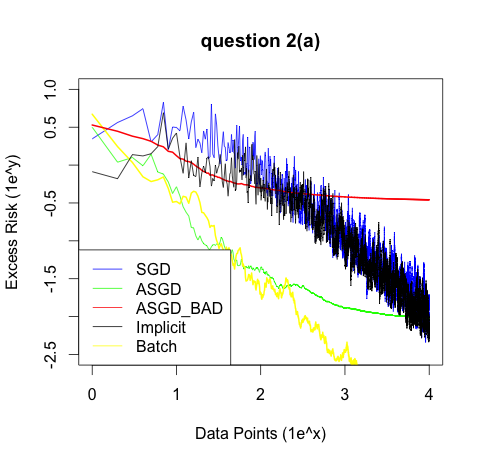
\includegraphics[width=400px]{2a.png}
      \item For SGD and implicit, we use a learning rate $a_t$ of $\gamma_0 * (1 + \gamma_0 \lambda_0 t)^{-1}$ and for ASGD we use $\gamma_0 * (1 + \gamma_0 \lambda_0 t)^{-2/3}$. Where $\gamma_0 = tr(A)$ and $\lambda_0 = .01$. \\
        \begin{align*}
          \text{ SGD: } \theta_{t+1} &= \theta_t - a_t * x^T\theta_tx + a_t * y * x \\
          \text{ ASGD: } \overline{\theta}_{t+1} &= (1 - 1/t)*\overline{ \theta }_t + (1/t)*\theta_{t+1} \\
          \text{ Implicit: } \theta_{t+1} &= \theta_t - a_t f_t x^T \theta_t x + a_t y x - a_t^2 f_t y \Sigma(x^2) x\\
            & \text{ where: } f_t = 1 / (1 + a_t \Sigma(x^2) ) \\
            & \text{ Note: this is taken from Panos' distro code } \\
          \text{ Batch: } & \text{ We ran the linear regression using R's lm(y } \sim \text{ x + 0) } \\
        \end{align*}
        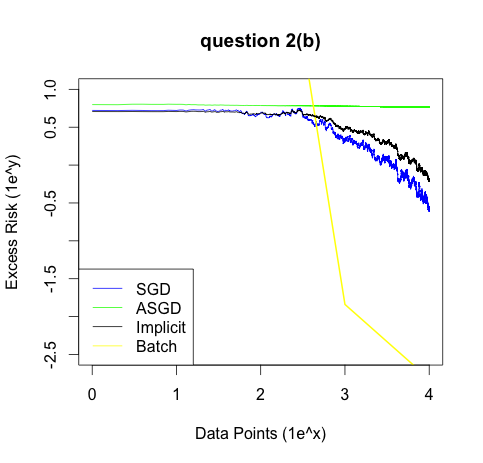
\includegraphics[width=400px]{2b.png}
        Note: After trying multiple learning rates and averaging rates for ASGD, for some reason we were still unable to produce the correct convergence rate. It may be some misunderstanding on our part or simply a bug in the code, but this will affect also 2(c).
    \end{enumerate}
   \item Part 3
      \begin{table}[!htbp] \centering 
  \caption{N = 1000, p = 100} 
  \label{} 
\begin{tabular}{@{\extracolsep{5pt}} ccccccc} 
\\[-1.8ex]\hline 
\hline \\[-1.8ex] 
 & 0 & 0.1 & 0.2 & 0.5 & 0.9 & 0.95 \\ 
\hline \\[-1.8ex] 
glmnet (type = "naive") & $0.035$ & $0.037$ & $0.041$ & $0.058$ & $0.144$ & $0.249$ \\ 
glmnet (type = "cov") & $0.010$ & $0.011$ & $0.011$ & $0.011$ & $0.017$ & $0.021$ \\ 
lars & $0.210$ & $0.207$ & $0.216$ & $0.214$ & $0.210$ & $0.213$ \\ 
\hline \\[-1.8ex] 
\end{tabular} 
\end{table}   

	  \begin{table}[!htbp] \centering 
  \caption{N = 5000, p = 100} 
  \label{} 
\begin{tabular}{@{\extracolsep{5pt}} ccccccc} 
\\[-1.8ex]\hline 
\hline \\[-1.8ex] 
 & 0 & 0.1 & 0.2 & 0.5 & 0.9 & 0.95 \\ 
\hline \\[-1.8ex] 
glmnet (type = "naive") & $0.129$ & $0.129$ & $0.148$ & $0.192$ & $0.480$ & $0.804$ \\ 
glmnet (type = "cov") & $0.033$ & $0.034$ & $0.032$ & $0.035$ & $0.038$ & $0.039$ \\ 
lars & $1.023$ & $1.053$ & $1.036$ & $1.047$ & $1.038$ & $1.029$ \\ 
\hline \\[-1.8ex] 
\end{tabular} 
\end{table}

	  \begin{table}[!htbp] \centering 
  \caption{N = 100, p = 1000} 
  \label{} 
\begin{tabular}{@{\extracolsep{5pt}} ccccccc} 
\\[-1.8ex]\hline 
\hline \\[-1.8ex] 
 & 0 & 0.1 & 0.2 & 0.5 & 0.9 & 0.95 \\ 
\hline \\[-1.8ex] 
glmnet (type = "naive") & $0.026$ & $0.024$ & $0.025$ & $0.030$ & $0.048$ & $0.051$ \\ 
glmnet (type = "cov") & $0.047$ & $0.045$ & $0.051$ & $0.070$ & $0.151$ & $0.136$ \\ 
lars & $0.319$ & $0.296$ & $0.303$ & $0.288$ & $0.306$ & $0.327$ \\ 
\hline \\[-1.8ex] 
\end{tabular} 
\end{table}    
   
	   \begin{table}[!htbp] \centering 
  \caption{N = 100, p = 5000} 
  \label{} 
\begin{tabular}{@{\extracolsep{5pt}} ccccccc} 
\\[-1.8ex]\hline 
\hline \\[-1.8ex] 
 & 0 & 0.1 & 0.2 & 0.5 & 0.9 & 0.95 \\ 
\hline \\[-1.8ex] 
glmnet (type = "naive") & $0.073$ & $0.075$ & $0.073$ & $0.086$ & $0.110$ & $0.194$ \\ 
glmnet (type = "cov") & $0.237$ & $0.257$ & $0.256$ & $0.312$ & $0.655$ & $0.679$ \\ 
lars & $1.893$ & $1.658$ & $1.619$ & $1.694$ & $1.758$ & $1.578$ \\ 
\hline \\[-1.8ex] 
\end{tabular} 
\end{table}    
   
		\begin{table}[!htbp] \centering 
  \caption{N = 100, p = 20000} 
  \label{} 
\begin{tabular}{@{\extracolsep{5pt}} ccccccc} 
\\[-1.8ex]\hline 
\hline \\[-1.8ex] 
 & 0 & 0.1 & 0.2 & 0.5 & 0.9 & 0.95 \\ 
\hline \\[-1.8ex] 
glmnet (type = "naive") & $0.264$ & $0.268$ & $0.269$ & $0.288$ & $0.347$ & $0.528$ \\ 
glmnet (type = "cov") & $0.981$ & $1.034$ & $1.069$ & $1.267$ & $2.348$ & $2.777$ \\ 
lars & $6.854$ & $7.487$ & $7.398$ & $7.351$ & $8.118$ & $7.584$ \\ 
\hline \\[-1.8ex] 
\end{tabular} 
\end{table}    

		\begin{table}[!htbp] \centering 
  \caption{N = 100, p = 50000} 
  \label{} 
\begin{tabular}{@{\extracolsep{5pt}} ccccccc} 
\\[-1.8ex]\hline 
\hline \\[-1.8ex] 
 & 0 & 0.1 & 0.2 & 0.5 & 0.9 & 0.95 \\ 
\hline \\[-1.8ex] 
glmnet (type = "naive") & $0.657$ & $0.714$ & $0.731$ & $0.722$ & $0.839$ & $1.598$ \\ 
glmnet (type = "cov") & $2.566$ & $2.666$ & $2.536$ & $3.227$ & $6.326$ & $8.347$ \\ 
lars & $22.491$ & $22.561$ & $25.666$ & $25.018$ & $23.115$ & $24.605$ \\ 
\hline \\[-1.8ex] 
\end{tabular} 
\end{table}    
\end{enumerate}
\end{document}
